% !TEX TS-program = pdflatex
% !TEX encoding = UTF-8 Unicode

\documentclass[a4paper, titlepage=false, parskip=full-, 10pt]{scrartcl}

\usepackage[utf8]{inputenc}
\usepackage[T1]{fontenc}
\usepackage[english, ngerman]{babel}
\usepackage{babelbib}
\usepackage{hyperref}
\usepackage{listings}
\usepackage{framed}
\usepackage{color}
\usepackage{graphicx}
\usepackage[normalem]{ulem}
\usepackage{cancel}
\usepackage{array}
\usepackage{amsmath}
\usepackage{amssymb}
\usepackage{amsthm}
\usepackage{algorithm}
\usepackage{algorithmic}
\usepackage{geometry}
\usepackage{subfigure}
\geometry{a4paper, top=20mm, left=35mm, right=25mm, bottom=40mm}

\newcounter{tasknbr}
\setcounter{tasknbr}{1}
\newenvironment{task}[1]{{\bf Aufgabe \arabic {tasknbr}\stepcounter{tasknbr}} (#1):\begin{enumerate}}{\end{enumerate}}
\newcommand{\subtask}[1]{\item[#1)]}

% Listings -----------------------------------------------------------------------------
\definecolor{red}{rgb}{.8,.1,.2}
\definecolor{blue}{rgb}{.2,.3,.7}
\definecolor{lightyellow}{rgb}{1.,1.,.97}
\definecolor{gray}{rgb}{.7,.7,.7}
\definecolor{darkgreen}{rgb}{0,.5,.1}
\definecolor{darkyellow}{rgb}{1.,.7,.3}
\lstloadlanguages{C++,[Objective]C,Java}
\lstset{
escapeinside={§§}{§§},
basicstyle=\ttfamily\footnotesize\mdseries,
columns=fullflexible,
keywordstyle=\bfseries\color{blue},
commentstyle=\color{darkgreen},      
stringstyle=\color{red},
numbers=left,
numberstyle=\ttfamily\scriptsize\color{gray},
breaklines=true,
showstringspaces=false,
tabsize=4,
captionpos=b,
float=htb,
frame=tb,
frameshape={RYR}{y}{y}{RYR},
rulecolor=\color{black},
xleftmargin=15pt,
xrightmargin=4pt,
aboveskip=\bigskipamount,
belowskip=\bigskipamount,
backgroundcolor=\color{lightyellow},
extendedchars=true,
belowcaptionskip=15pt}

%% Enter current values here: %%
\newcommand{\lecture}{Robotik WS15/16}
\newcommand{\tutor}{}
\newcommand{\assignmentnbr}{6}
\newcommand{\students}{Julius Auer, Thomas Tegethoff}
%%-------------------------------------%%

\begin{document}  
{\small \textsl{\lecture \hfill \tutor}}
\hrule
\begin{center}
\textbf{Übungsblatt \assignmentnbr}\\
[\bigskipamount]
{\small \students}
\end{center}
\hrule

\begin{task}{Inverse Kinematik}
\item[]
Die Rechnung auf den Folien ist leider nicht korrekt (?) - die Matrizen sind etwas komplexer:

\begin{align*}
T_{2\rightarrow 0}&=\begin{pmatrix}c_1&-s_1&0\\s_1&c_1&0\\0&0&1\end{pmatrix}\cdot\begin{pmatrix}c_2&-s_2&l_1\\s_2&c_2&0\\0&0&1\end{pmatrix}\text{(soweit, so gut. Aber:)}\\
\begin{pmatrix}x\\y\\1\end{pmatrix}&=\begin{pmatrix}c_1&-s_1&0\\s_1&c_1&0\\0&0&1\end{pmatrix}\cdot\begin{pmatrix}c_2&-s_2&l_1\\s_2&c_2&0\\0&0&1\end{pmatrix}\cdot\begin{pmatrix}l_2\\0\\1\end{pmatrix}\\
&=\begin{pmatrix}c_1&-s_1&0\\s_1&c_1&0\\0&0&1\end{pmatrix}\cdot\begin{pmatrix}l_2\cdot c_2+l_1\\l_2\cdot s_2\\1\end{pmatrix}\\
&=\begin{pmatrix}l_1\cdot c_1+l_2\cdot (c_1\cdot c_2-s_1\cdot s_2)\\l_1\cdot s_1+l_2\cdot (s_1\cdot c_2+c_1\cdot s_2)\\1\end{pmatrix}\\
\frac{\delta}{\delta\Theta_1}\begin{pmatrix}x\\y\\1\end{pmatrix}&=\begin{pmatrix}-l_1\cdot s_1+l_2\cdot (-s_1\cdot c_2-c_1\cdot s_2)\\l_1\cdot c_1+l_2\cdot (c_1\cdot c_2-s_1\cdot s_2)\\0\end{pmatrix}\\
\frac{\delta}{\delta\Theta_2}\begin{pmatrix}x\\y\\1\end{pmatrix}&=\begin{pmatrix}l_2\cdot (-c_1\cdot s_2-s_1\cdot c_2)\\l_2\cdot (-s_1\cdot s_2+c_1\cdot c_2)\\0\end{pmatrix}\\
J&=\begin{pmatrix}-l_1\cdot s_1+l_2\cdot (-s_1\cdot c_2-c_1\cdot s_2)&l_2\cdot (-c_1\cdot s_2-s_1\cdot c_2)\\l_1\cdot c_1+l_2\cdot (c_1\cdot c_2-s_1\cdot s_2)&l_2\cdot (-s_1\cdot s_2+c_1\cdot c_2)\end{pmatrix}\\
&=\begin{pmatrix}-y&l_2\cdot (-c_1\cdot s_2-s_1\cdot c_2)\\x&l_2\cdot (-s_1\cdot s_2+c_1\cdot c_2)\end{pmatrix}
\end{align*}

Da die Jakobi-Matrix hier immer hübsch quadratisch ist, kann die Inverse direkt über die geschlossene Form berechnet werden:

\begin{align*}
J^{-1}&=\frac{1}{l_1\cdot l_2\cdot (s_1^2\cdot s_2+c_1^2\cdot s_2)}\cdot\begin{pmatrix}l_2\cdot (-s_1\cdot s_2+c_1\cdot c_2)&-l_2\cdot (-c_1\cdot s_2-s_1\cdot c_2)\\-l_1\cdot c_1-l_2\cdot (c_1\cdot c_2-s_1\cdot s_2)&-l_1\cdot s_1+l_2\cdot (-s_1\cdot c_2-c_1\cdot s_2)\end{pmatrix}
\end{align*}

Es seien nun: $l_1,l_2$ fest, $tf(\Theta_1,\Theta_2):\mathbb{R}\times\mathbb{R}\rightarrow\mathbb{R}^2$ eine Funktion um wie gezeigt $T_{2\rightarrow 0}$ zu erzeugen, $j(\Theta_1,\Theta_2):\mathbb{R^2}\rightarrow\mathbb{R}^{2\times 2}$ eine Funktion um wie gezeigt $J^{-1}$ zu erzeugen, $f(\overrightarrow{x}):\mathbb{R}^2\rightarrow\mathbb{B}$ eine Funktion die bei Eingabe der aktuellen Position $\overrightarrow{x}$ entscheidet ob der Algorithmus terminiert und $d\in\left[ 0,1\right] $ ein Dämpfungsfaktor. Dann lässt sich die inverse Kinematik folgenderweise berechnen:

\newpage
\begin{enumerate}
\item[(1)]Initiale Winkel: $\Theta_1,\Theta_2$
\item[(2)]End-Effektor-Position: $\overrightarrow{x}=tf(\Theta_1,\Theta_2)$
\item[(3)]Ziel-Position: $\overrightarrow{x_t}$
\item[(4)]solange $f(\overrightarrow{x})$:
\begin{enumerate}
\item[(5)]Prüfe und behandle ggf. Singularität (tritt hier nicht auf, falls Anfangsposition günstig gewählt)
\item[(6)]$\begin{pmatrix}\Theta_1\\\Theta_2\end{pmatrix}+=d\cdot j(\Theta_1,\Theta_2)\cdot (\overrightarrow{x_t}-\overrightarrow{x})$
\item[(7)]$\overrightarrow{x}=tf(\Theta_1,\Theta_2)$
\end{enumerate}
\end{enumerate}

Genauso implementiert liefert das die folgenden Ergebnisse:

\begin{figure}[!htpb]
\begin{center}
\subfigure[Plot]{
  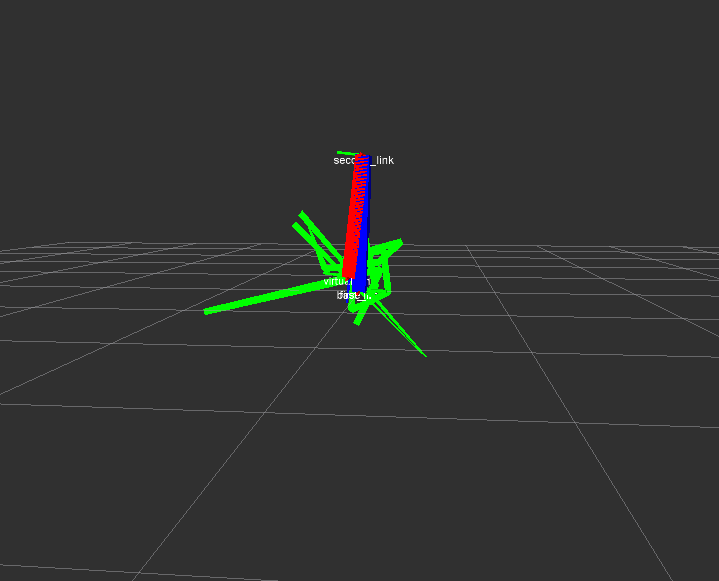
\includegraphics[width=0.49\linewidth]{capture_1-1}
}
\subfigure[Trajektorie]{
  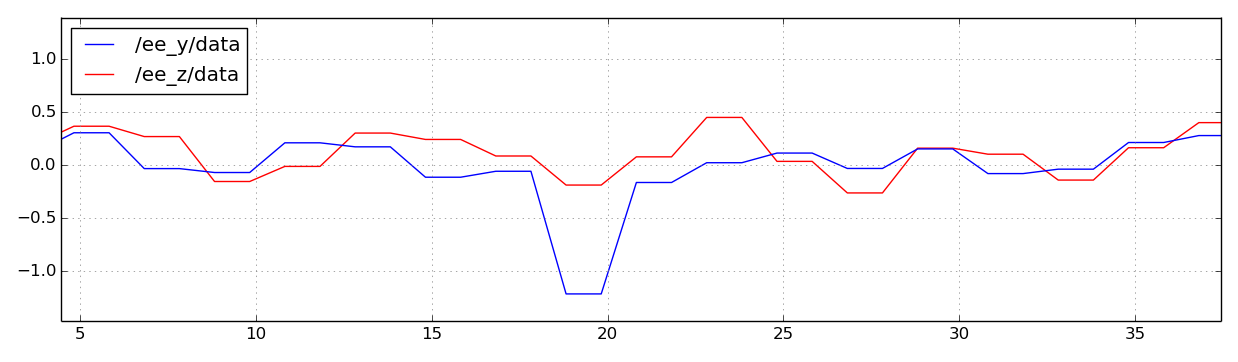
\includegraphics[width=0.49\linewidth]{capture_1-2}
}
\end{center}
\caption{1 Iteration}
\end{figure}

\subtask{b}
\begin{figure}[!htpb]
\begin{center}
\subfigure[Plot]{
  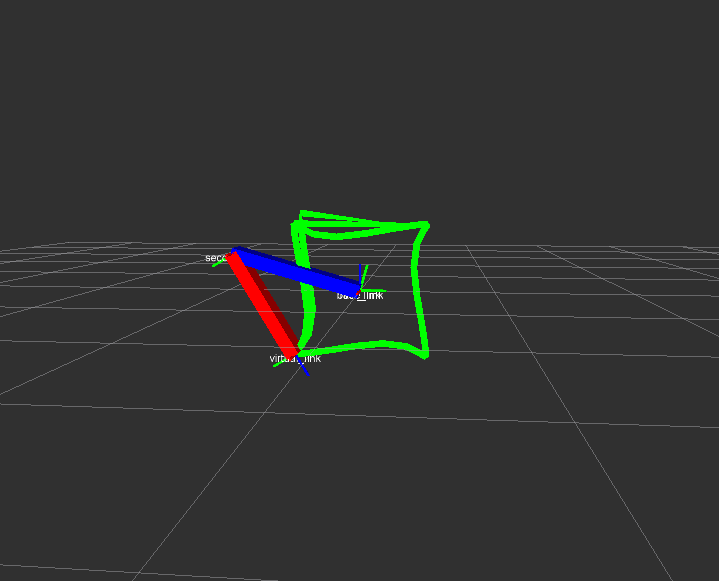
\includegraphics[width=0.49\linewidth]{capture_1-3}
}
\subfigure[Trajektorie]{
  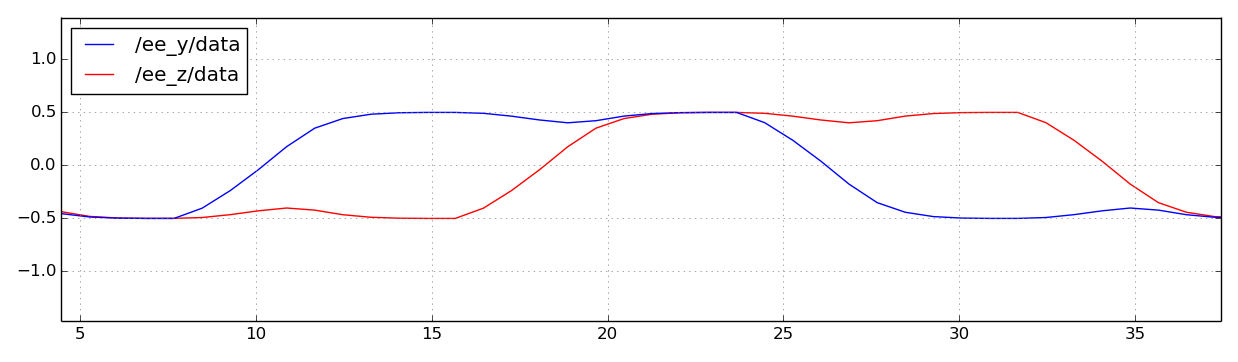
\includegraphics[width=0.49\linewidth]{capture_1-4}
}
\end{center}
\caption{10 Iteration}
\end{figure}

\subtask{c}
\begin{figure}[!htpb]
\begin{center}
\subfigure[Plot]{
  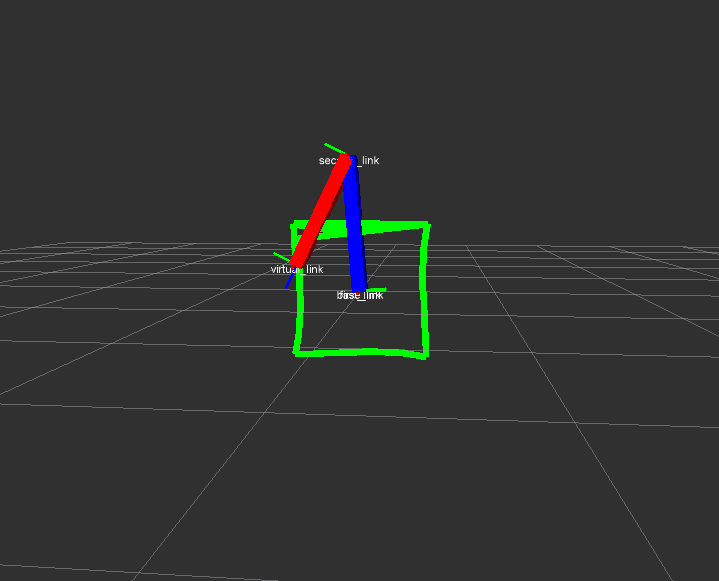
\includegraphics[width=0.49\linewidth]{capture_1-5}
}
\subfigure[Trajektorie]{
  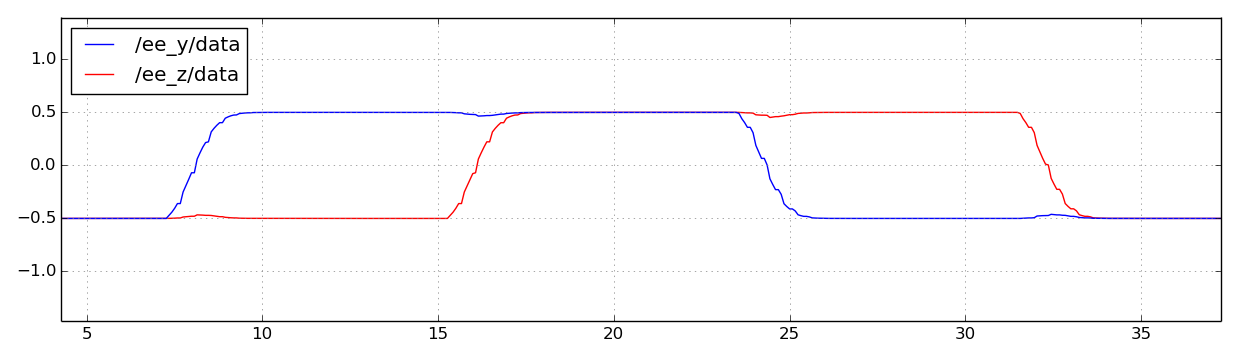
\includegraphics[width=0.49\linewidth]{capture_1-6}
}
\end{center}
\caption{100 Iteration}
\end{figure}

\subtask{d}
\begin{figure}[!htpb]
\begin{center}
\subfigure[Plot]{
  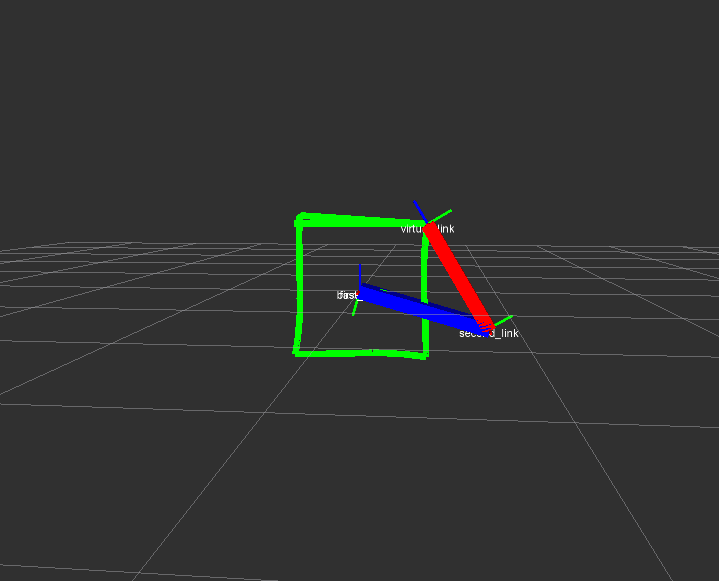
\includegraphics[width=0.49\linewidth]{capture_1-7}
}
\subfigure[Trajektorie]{
  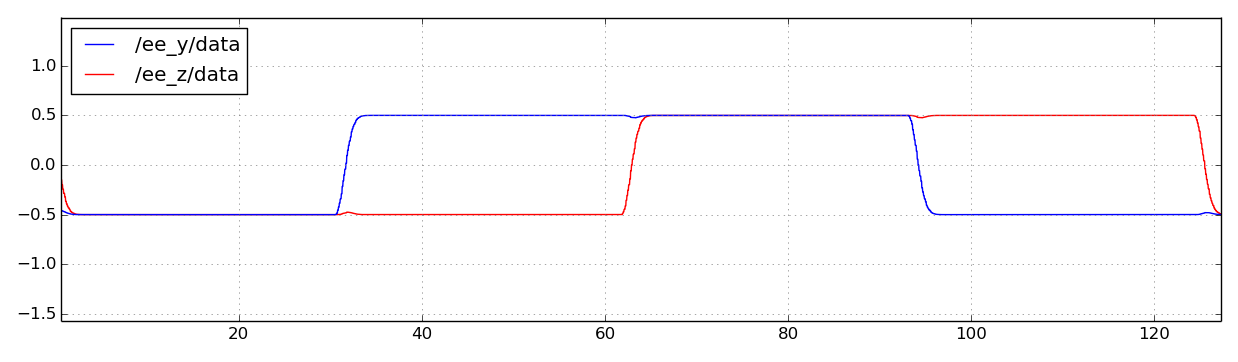
\includegraphics[width=0.49\linewidth]{capture_1-8}
}
\end{center}
\caption{1000 Iteration}
\end{figure}

\end{task}

\begin{task}{Null-Space}
\item[]

\end{task}
\end{document}